% Sequence Diagrams: http://ftp.fau.de/ctan/graphics/pgf/contrib/pgf-umlsd/pgf-umlsd-manual.pdf

\documentclass{scrartcl}
 \setlength\parindent{0pt}
\usepackage[utf8]{inputenc}
\usepackage[T1]{fontenc}
\usepackage{lmodern}
\usepackage{amsmath}
\PassOptionsToPackage{hyphens}{url}\usepackage{hyperref}
\usepackage{graphicx}
\usepackage{listing}
\usepackage{amssymb}
\usepackage{listings}

\usepackage{pgf-umlsd}



\usepackage[style=numeric,backend=bibtex]{biblatex}
\addbibresource{references.bib}

\lstdefinestyle{JSON2}
{
    language=JSON,
    literate = *{\ \ }{\ }1, %replaces each occurence of two consecutive spaces by one
}

\usepackage{tikz}
\usetikzlibrary{matrix,shapes,arrows,positioning,chains, calc}

 \PassOptionsToPackage{hyphens}{url}\usepackage{hyperref} %make url break
\title{Charme: A distributed social network with end-to-end encryption and contextual information (DRAFT)}
\author{Manuel Schultheiß\\manuel.schultheiss@tum.de}
\begin{document}  \sloppy % sloppy is used for making url{} break
 
\maketitle

\begin{abstract}
\noindent
  \textbf{Abstract.} 
  Decentralized social networks with end-to-end encryption would take back control of data to the end-users. In this paper Charme is presented as such a network. First, some  basic cryptographic  principles are explained before focusing on the underlying  protocol.
  \end{abstract}
  
  
\tableofcontents
 \newpage
\section{Prologue}

\begin{center}
\textit{I's personal. It's private.
And it's no one's business but yours.}
\end{center}

These are the first words, of Phil Zimmermann's essay "Why I wrote PGP" from 1991 \cite{PHIL}, arguing why emails should remain private. 24 year later, electronic communication has gained more and more attention in your everyday life. Today, letters have become instant messages and half of your real world conversations have become social network posts. But while you could be almost sure a letter remained private, today a bunch of stakeholders such as governments, technicians and ad-serving companies has access to data derived from your conversations. \\


Most people give a "I have nothing to hide" as an answer when addressing this point. Regarding confidentiality may be true, as long as you are not a politician, your are not responsible for a business unit, or do not have anything else to say other people are willing to listen to. But while your self forgets most of the things you said, it is probably saved in some data center waiting to get parsed by some algorithms. With more and more data you become calculable, your actions, - like what products you are willing buy or who do you vote for - can be predicted and influenced long before you perform them.\\


But beside ads have become the number one revenue model for internet companies and politicians and trying to expand data collection  whenever it is possible \cite{EFF}, there is also one more problem: With the decay of classic media, such as newspaper and television, social networks have become the primary infrastructure of directing people to information now. The heterogeneous  landscape of newspapers and blogs providing different information is slowly fading. The newsfeed has become the primary source of information. And it is not  wise to trust a single institution  here, because who controls what you read controls who you become.






\newpage
\section{Introduction}
In contrast to classic social networks, distributed social networks with end-to-end encryption can provide self control of your data and  independence from big companies.  \textit{Distributed} means, that there is no central server hosting your data, but many small servers all around the world, which everyone can  setup. Just like email, every participant has a unique address like \textit{yourname@yourserver.com}. With end-to-end encryption not even the server hosting your data can see your data. This is necessary for a distributed architecture as otherwise the server admin could read your messages, for example.\\

Another innovation of Charme is the so called \textit{Context}, every post can have optionally. A context contains semantic, computer-readable information about the post.
 An algorithm can later aggregate all people moving from point A to point B tomorrow, with having 3 seats free in their car with a tolerance of 20 kilometers, for example. Or you can look up for friends making pizza for lunch and want to share their food today. Figure \ref{figContext} shows the creation of a context and the creation of a filter to search for existing context of other users. 
 Websites already providing share-economy services can also add their data to the Charme network, using the Charme Schema JSON Syntax, as defined in the file schema.coffee. The context system introduces elements of the \textit{Web of Data}, formerly known as the semantic web to social networks.

\begin{figure}[ht]
	\centering
  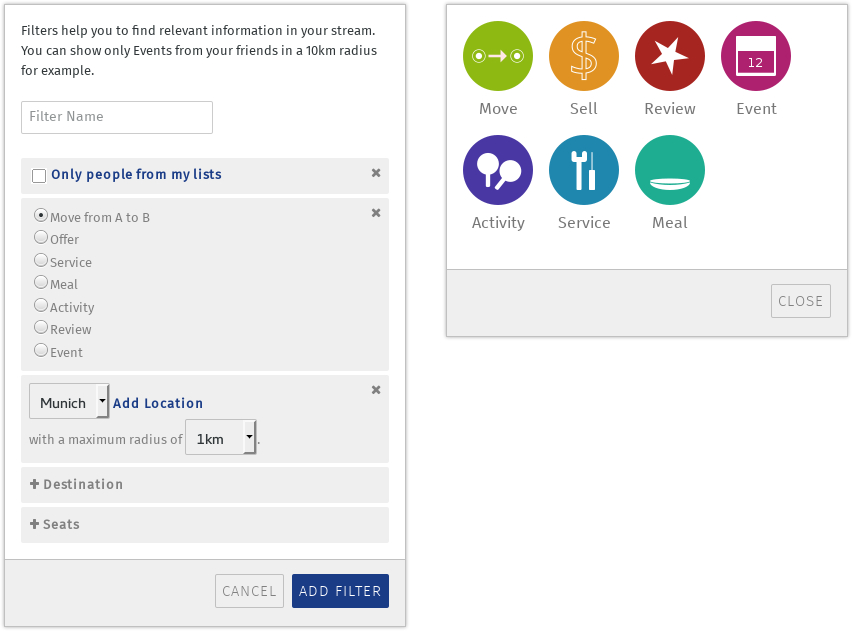
\includegraphics[width=90mm]{illustrations/context.jpg}
	\caption{Context dialogues. Search dialogue on the left; Create dialogue on the right. You can perform searches for transportation, events, products, ride sharing and activities for example.}
	\label{figContext}
\end{figure}
\newpage
 \section{Existing work}
With Diaspora \cite{diaspora}, one of the first popular distributed social networks was released. The messages are not end-to-end encrypted, however, which makes it possible for the server admin to read its users messages. 
A more secure concept is \textit{Twister} \cite{twister}, a Twitter like peer-to-peer micro blogging platform. Using the blockchain makes it possible to encrypt messages and even meta data (including the IP Address!). Charme itself does not encrypt meta data at the moment for simplicity and performance reasons, but such an encryption scheme could be implemented later on using techniques like onion routing between sender/receiver for example.

\newpage
 \section{Encryption and Security}

\subsection{Formal Notation used in this paper}
\subsubsection{Reach}
 We define the \textit{reach} of a server: Each server $S_i$, on which at least one user has a public key of another user hosted on server $T_j$ with $i,j \in {0,1,2,..}$ is \textit{reached} by this server.
The reach is a list of tuples $(S_i, T_j)$. See figure \ref{figContextGraph} as an example.

\begin{figure}[ht]
	\centering
    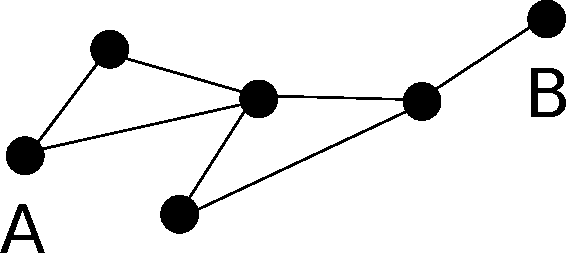
\includegraphics[width=30mm]{illustrations/graph.pdf}

	\caption{$|Reach(A)| = deg(A) = 2
$ as the users on server A have public keys of two different servers. The bidirectional edges representing two servers having public keys of users on the respectively other server (In a real world scenario, there would be some directed edges of course). }
	\label{figContextGraph}
\end{figure}





 
\subsection{Cryptographic Primitives}
\subsubsection{AES-CBC \label{AESCBC}}
AES is a fast, symmetric encryption algorithm that was standardized in 2001 and is still considered secure, although there exist some attacks on it. The following explanation is based on the lecture slides of Carle et al \cite{carle}.

A key $K_{A,B}$ is used for encryption and decryption by the two parties A and B. 
Cipher Block Chaining Mode (CBC) ensures that blocks that are identical in the plaintext, are not identical anymore in the chiphertext. This is essential, as otherwise images can still be recognized for example, although they are encrypted. First, a initialization vector (IV) is created:
$$
c_0 = IV
$$

A plaintext block $p_i$ becomes a chipher block $c_i$ during encryption.
$$
c_i = Enc_K(c_{i-1} \oplus p_i)
$$
and the same thing reversed for decryption:
$$
p_i = c_{i-1} \oplus Dec_K(K, c_i)
$$
It is important that the IV is shipped with integrity protection, otherwise an attacker could modify the first 256 bits in order to set the first decrypted plaintext block to a custom value. The other blocks can not be influenced however. 
There are several techniques to add it (
\url{https://en.wikipedia.org/wiki/Authenticated_encryption}).
 Integrity protection can be achieved using the following steps using an encrypt-then-mac Scheme:
\begin{enumerate}
\item Encrypt Message using AES-CBC
\item Get SHA-256 hash value of encrypted message and salt with key k and crypto algorithm version a.
\item JSON Result is:
\begin{lstlisting}[mathescape]
 { 
   a: 1,
   m: $Enc_{k||v}(text)$,
   h: $HMAC_{Sha256}$($Enc_{k||v}$(text), $k||v$)
 }
 \end{lstlisting}
  The algorithm version a is added, as otherwise, an attacker could extract the plaintext and use backwards compatibility to let the decryption and MAC check be performed by an old algorithm, also there is a better algorithm available.

For example: The current implementation supports Non-HMAC AES when the information was encrypted without a HMAC. An attacker could remove the HMAC key and just send the plain AES encrypted content to the client and the client would still decrypt it correctly.

\end{enumerate}
Please note that for more security, the salt for the $HMAC_{Sha256}$ should also not use k, but a derived version of k.

\subsubsection{RSA}
In RSA there are two different keys. The public key is visible to everyone, while the private key is only visible to the \textit{generator} of both keys. The public key can be used by anyone to send the \textit{generator} a message, while the private key can used by the \textit{generator} to decrypt the message. Asymmetric encryption is a lot of slower than symmetric encryption. So usually we generate an AES key, encrypt the text with the AES key and encrypt the AES key with the RSA key, rather than encrypting the whole text with the RSA key.
For RSA, we generate two large prime numbers $p$ and $q$.
\begin{eqnarray*}
 n = p *q 
\end{eqnarray*}
 and define
\begin{eqnarray*}
 \Phi(n) = (p-1)*(q-1)
\end{eqnarray*}
 Let e not equal to 1, smaller than $ \Phi(n)$ and not share a common divisor with $ \Phi(n)$.
 Now we compute d under the restriction:
 \newcommand{\Mod}[1]{\ (\text{mod}\ #1)}
\begin{eqnarray*}
 e*d = 1 \Mod{\Phi(n)}
\end{eqnarray*}
 To encrypt a message M or decrypt chipher C use:
\begin{eqnarray*}
 C = M^e \Mod{n}\\
 M = C^d \Mod{n}
\end{eqnarray*}
 To provide \textit{Ciphertext indistinguishability} RSA is used with a padding scheme like PKCS1. Here we generate n with more than two primes:
 \begin{eqnarray*}
 n = p_1*p_2*...*p_n
\end{eqnarray*}
with $p_1$ being r and $p_2$ being $q$.
\cite{carle}
 % TUM Network Security, WS 2014/15, Chapter 2.4 The RSA Public Key Algorithm

\subsubsection{Further reading}
\begin{enumerate}
\item PKCS\#1 v2.2 RSA Cryptography Standard\\\url{http://www.emc.com/collateral/white-papers/h11300-pkcs-1v2-2-rsa-cryptography-standard-wp.pdf} 
\item Lessons learned and misconceptions regarding encryption and cryptology \\\url{
http://security.stackexchange.com/questions/2202/lessons-learned-and-misconceptions-regarding-encryption-and-cryptology/2206#2206}
\item HMAC versus raw SHA hash functions \\\url{
http://dev.ionous.net/2009/03/hmac-vs-raw-sha-1.html}
\end{enumerate}


\subsection{Used Libraries}
There are a Javascript library called Gibberish AES for Javascript and Tom Wu's RSA Library for RSA providing the main functionality in the technology preview. Google wrote with its E2E project a better implementation of cryptographic algorithms which should replace the above ones as soon as possible. The long term goal is to use the W3C web crypto API however, if supported in all major browsers, as this one is more secure regarding key deletion from memory (RAM) and random number generation. 

\newpage
\section{Implementation}
\subsection{Backend Technology Stack}
The current implementation is a proof-of-concept, which means it is not ready for production use yet.
On server side, PHP is used as an interpreter. The reason for PHP is that it has a wide community supporting it, as it is used by many other big websites like Facebook or Wordpress for example. Furthermore it does not depend on 100 extra packages for basic functions with questionable future support like Node.js.
 \textit{ZeroMQ} is used to send socket messages and communicate between different PHP threads. \textit{Gearman} is necessary to execute background tasks like sending messages in the asynchronously. As a database, \textit{MongoDB} is used, as it is scalable and has the ability to directly store JSON object to the database.
Administrations scripts are written for GNU Bash to provide easy ssh access.



 \subsection{Separation of Client and Server}
In contrast to classic social networks, we separate client and server in two separate projects first. In Charme, the server does not return HTML to the browser, but JSON instead which is parsed by the client software. This is necessary, as otherwise a server could return malicious javascript to the user for example and make end-to-end encryption useless. For the final release, the user has to download and install the client locally and verify the file hash to have maximum security, For testing purposes, the user can also use a web hosted version of the client. Although they are hosted on different domains, client and server can still connect to each other via cross origin resource sharing (CORS).

\begin{figure}[ht]
	\centering
  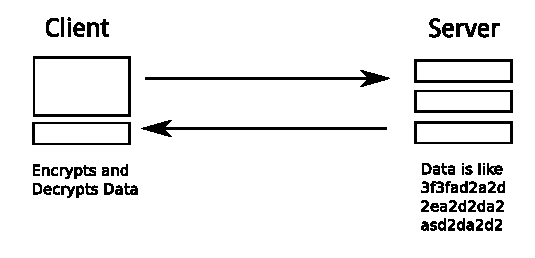
\includegraphics[]{eds.pdf}
	\caption{Client and Server code is strictly separated. The client loads the Charme application from a local webserver, a browser plugin or a trusted server. This application connects to the server that is hosting the user's data itself. Hereby, personal data such as messages or private profile information, is encrypted and decrypted on the client side, so the server sees nothing.}
	\label{fig1}
\end{figure}


Hereby Charme uses an \textit{encrypted data storage}. This means critical data is encryped with a passhprase using AES-CBC (Section \ref{AESCBC}) and hosted on the server  (Figure \ref{fig1}). Consequently the server can not read the encrypted user data. Such data includes
\begin{enumerate}
\item \textbf{Personal information} like phone number. This information can later be decrypted and encrypted with a public key to distribute it to other people.
\item \textbf{The private RSA key} used to decrypt everything that is received from other users.
\item \textbf{The key directory}, which contains the public keys of all contacts. Here it is important that the receiver B of a message sent by user A only uses the newest private key to decrypt, as a malicious server of the key directory owner could return an old public key of user B.
\end{enumerate}
for example. The data must also be signed to prevent manipulation such as bit flipping etc.

\subsection{Public Keys Verification}
If we want to send an encrypted message to user B, we need the public key of user B first. However, as an evil server or a man-in-the-middle can provide a wrong public key, it is necessary to check the public key for correctness. If done so, we encrypt the public key of user B with our passphrase and store it in the encrypted data storage.
 

The user itself has to validate the fingerprint. Currently the fingerprint $f$ is generated by applying a SHA-256 Hash function on n (modulus) and e (exponent) of the RSA key concatenated:
   $$
   F = Sha256(n || e)
   $$
 For a better user experience, the fingerprint can be truncated and  seperated by ":", so the result looks something like:
  
   \begin{center}
   12 : 3f : 3e : 2f: 12 : 3f : 3e : 2f: 12 : 3f : 3e : 2f (...)
   \end{center}
  
  instead of 
  
  \begin{center}
  123f3e3f123f3e2f123f3e2f (...)
  \end{center}
  
  Fingerprints are used to verify public keys of other users.
  Figure \ref{figFP} shows the dialog to validate fingerprints.\\
  
  \begin{figure}[ht]
	\centering
  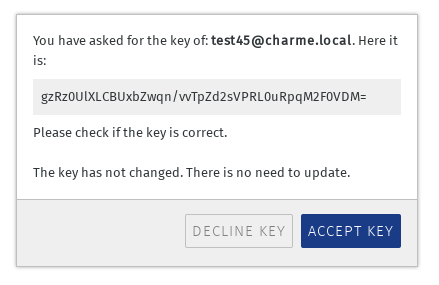
\includegraphics[width=90mm]{illustrations/fingerprint.png}
	\caption{Fingerprint Validation Dialog}
	\label{figFP}
\end{figure}


One thing that is missing right now is to make sure that the \textbf{server always returns the newest verified public key} of a user. Hereby an evil server could provide an old, compromised key. So we got two things to fix here:
\begin{enumerate}
\item Other users should not see messages or parse  control messages, which were encrypted with an old key, as such messages may have been faked.
\item A man in the middle (MITM) should not be able to provide an old public key and read messages exchanged between two users. See figure \ref{figkp} for an example attack. This attack requires a malicious host server however, as we assume the protocol between client and server is HTTPs. Furthermore it requires an old compromised key.
\end {enumerate}


  \begin{figure}[ht]




\begin{sequencediagram}
\newthread[white]{ac}{Client A}
\newinst[4]{mitm}{Man in the Middle}
\newinst[4]{as}{Server A}

\begin{call}{ac}{1. Get Public Key of A, Rev. 4}{mitm}{5. Return Public Key of A Rev. 3}

\begin{call}{mitm}{2. (...)}{as}{4. Return Public Key of A Rev. 4}
\end{call}

\end{call}

\begin{call}{ac}{6.Send message}{mitm}{8. ACK}

\mess{mitm}{7. Decrypt message}{mitm}


%\mess{a}{ message }{b}
\end{call}
 
\end{sequencediagram}


	\caption{MITM attack on keydirectory. A nonce between client and server is not solution as we also assume that the server A has been compromised.}
	\label{figkp}
	
\end{figure}



To fix  the \textbf{first vulnerability}, we have to take care about a few things:
\begin{description}
\item[Old Public Keys have to be rejected by server] If a message from server A is encrypted with an old public key, server B will drop it. A message from A to A can still be received by an evil server, however.

\item[Old Public keys have to be rejected by client] the client software must also drop messages that are not encrypted with the latest public key. To check this, we must add the creation time to each public key.


\end{description}

The \textbf{second vulnerability} (Figure \ref{figkp})is harder to fix. While we can store the newest key version on the client device, on which it was added to prevent MITM on this device, it is hard to notify the other devices about the newest key version. Example:
\begin{enumerate}
\item Newest key revision of B is 1
\item User A adds new key of user B on device 1. Device 1 knows newest key revision of B is 2
\item User A sends messages to user B on device 2. Uses revision 1 as told by MITM (Key directory replay attack) between client and server.
\item MITM can read message with compromised revision 1 key.
\end{enumerate}

The best practice would be to display a "security message" on all devices, which shows up after a key was added on another device:
\begin{enumerate}
\item User adds public key on device 1. Message is \textit{"Please check your Android device (device 2) for push notification about revision 2. If you do not receive this message your server is probably evil."}. We send control message $c = Enc_{fastkey1}(\lbrace userid, revision\rbrace )$ to our server who sends it to device 2.
\item  Device 2 can decrypt and display the message "User ... has new revision of ...". We also poll the new key directory from the server. The sum of public key revisions must be greater than it was before, otherwise an attack was performed. 
\item Additionally we have a security page, were the hash of the key directory is displayed, on each device.
\end{enumerate}


%One solution would be to display the sum of public key revisions in the key directory on each device somewhere, so the user can check that all keys are up-to-date and in the newest revision. However if device 1 and 2 add one different key parallel it is still the same , although having different keys.


%Messages can still be received by setting the date in the past and use an old public key, however. As an additional security feature, the newest key revision can be stored on client side. Here we run into a sync problem:
%\begin{enumerate}
%\item Newest key revision of B is 2
%\item User A adds new key of user B on device 1. Client knows newest key revision of B is 2
%\item User A sends messages to user B on device 2
%\item User B denies the message because key is to old
%\end{enumerate}
%We basically want to sync the public key, without verifying it again. So we send $Enc_{fastkey1}({userid, newestRevision})$ to the other devices which forces and update of the key storage.


  
 \subsection{Encryption}
The data to be encrypted can be divided into three main categories:

\begin{description}
  \item[Posts] Posts of collections are encrypted for a lot of users. Each post is encrypted with a key, which needs to be distributed to the audience of the post using public key cryptography.
  \item[Messages] Each message belongs to a conversation. Each conversation has a key, which needs to be distributed to the message receivers. Here we also have to take care of cases when someone is added and removed from a conversation.
  \item[Personal Information] such as phone number or hometown. Here we have to make sure, that if access is revoked, we do not have to generate a new key and distribute it to all people. Therefore we introduce buckets, which make it possible to handle this case more efficient.
\end{description}

The following sections will give a basic overview, for a more detailed explanation see section \ref{protocol}.
 \subsubsection{Edgekeys}
 An edgekey is a symmetric key, that is established after public key verification and encrypted via public key by the other party. This is done, because asymmetric cryptography is a lot of slower than symmetric cryptography.
 \subsubsection{Post Encryption}
A new post is encrypted, when its audience is restricted to a list of people. 
In this case we generate a postkey $pk$, which encrypts the content of the post. Next we need to distribute $k$ to other people. We can use the symmetric edgekeys $e_1, e_2, ...$ of these people to encrypt the postkeys: $k_{enc} = enc_{e_1} (k)$. Next we distribute it to the corresponding receivers. Furthermore we generate a signature of post data with our private key, and add the public key revision of the receiver.
 \subsubsection{Message Encryption}
 
  Message encryption is basically working like in PGP. A simplified concept is illustrated in Figure \ref{fig2}). 
To start a new converation we obtain the public keys of the receivers from the encrypted data storage first. Then we generate a symmetric key and distribute it to the receivers. The symmetric key can change if a user is removed or a public key of a conversation participant is updated or a certain span of time has passed. In this case, we have to distribute it again. A new message is encrypted with the newest symmetric key $s$.
A message consists of information such as \textit{message content}, \textit{conversation identifier}, \textit{time} and \textit{key identifier} of the symmetric key used for encryption. This information is  signed using the senders private key.

 \begin{figure}[ht]
	\centering
  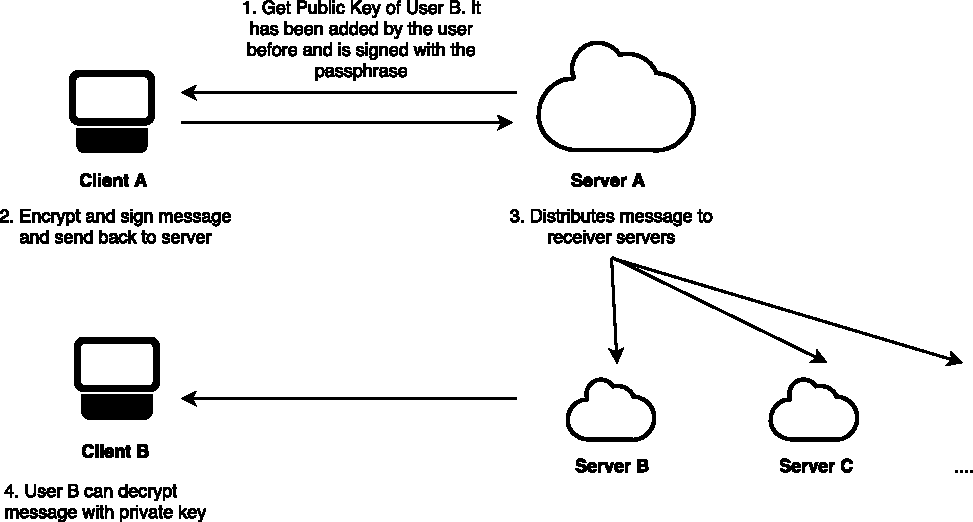
\includegraphics[width=120mm]{pubkey.pdf}
	\caption{Basic message encryption. Server A can also send the message to more servers than only Server B. The client does not send the message directly to server B, as with increasing number of receivers this would cost to much bandwidth for the client.}
	\label{fig2}
\end{figure}


  \subsubsection{Encryption of Personal Information}
  When disclosing private information like telephone number or email to other people, this is working slightly different to message distribution for performance reasons.  If the access to a certain person is revoked, it would be inefficient to send the new key to all users. Instead we create  \textit{buckets}, each containing a maximum of k users. When a new piece of information is encrypted, we generate a random key $K$, and encrypt it with the bucket key $B_i$. As every user who has access to the information, owns the bucket key, the user can decrypt it with
  $$
  plaintext = Dec_{B_i}({Dec_K(chiphertext)})
  $$
  When access is revoked for a user, we simply generate a new bucket key for the bucket assigned to the user and distribute the new bucket key to all users in this bucket. With this system we are able to revoke access to information and release new information to a user with doing $\mathcal O(k) = \mathcal O(1)$ requests. For Charme we set $k = 10$. See figure \ref{fig3} for a illustration of the process.
  
  
   \begin{figure}[ht]
	\centering
  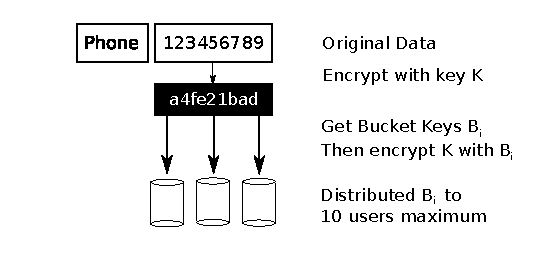
\includegraphics[]{prvInfo.pdf}
	\caption{Encryption of personal information using buckets}
	\label{fig3}
\end{figure}

    \subsection{Key Updates}
    When a private key or passphrase is compromised  it is necessary to recrypt the encryped data storage to protect it from future access by the attacker. In this case, all information is transmitted to the client, decryped with the current passphrase and encrypted with the new passhprase. The revision number for the public key increases afterwards. 

  \subsection{Primary Attack Vectors}
  
  \subsubsection{Data Integrity}
We must ensure, that the server can only return data, that has been created by a user. 
As an example, the autocomplete should only returns name/address pairs that have been added by the user. Imagine the following case: Alice adds Bob with his CharmeId bob@somewhere.com to her key directory. Now she wants to send a message to Bob and opens the auto complete. She types Bob, and the server returns a modified CharmeId, probably on the same server (eve@somewhere.com). The Charme client would now encrypt the message with the other key and send it to Eve. So Eve could be able to get some sensitive information while Alice thinks she is communicating with Bob.
Therefore we must sign most data with a pass phrase derived key.\\

  Also conversation messages itself must be shipped with integrity protection. In contrast to the above example, here we must protect the integrity for other users than our self.

When we use the conversation key for the hmac of the message, we only protect the message against attacker that are not part of the conversation. Let person A and B be part of one conversation. Now person A could still send messages with the name of person B. Using the private key would be a better solution here, but it is computationally expensive (aka slow, especially on mobile devices) to check a RSA signature in the background. It is probably the best idea to check use the first approach for a background verification and the second approach only after a click on a "Check signature" button. The second approach should also be used with a smaller RSA key length for background verification, however.


   

  \subsubsection{MITM on Client Software}
  The client software must be distributed with integrity protection in the final release. For example as a Apache Cordova package. To use the client software on a third party server is very dangerous and only recommended for testing purposes! The host of the client can theoretically read all your data by modifying the client software.
  
   There is also a new technology called sub resource integrity which can be used to validate Javascript and CSS resources (See \url{http://www.w3.org/TR/SRI/} and \url{http://githubengineering.com/subresource-integrity/}). Maybe they introduce some mechanism to validate a whole web page with a hash recommended by the majority of browser users and additionally located on a (Mozilla or Google) server. So lets keep an eye on that.


   
     \subsubsection{New Conversations with malicious userId/Name pair }
     An attacker can initiate a new conversation with the name of a friend of you, but use another userId instead. Example:
      \begin{enumerate}
     \item Alice (alice@server.com) and Bob Alice (bob@server.com) are friends
     \item Eve initiates a new conversation with Bob with Name "Alice" and userId eve@server.com. 
     \item Bob thinks he is talking to Alice, but he is not.
     \end{enumerate}
     A solution for this problem would be to allow only names from the key directory.
   \subsubsection{XSS}
   One of the most critical attack vectors in Charme is Cross Site Scripting as with this technique private keys can be stolen.
   Therefore it is important to sanitize all displayed data from other people and servers. Never trust the server. For example imaging data is a JSON Object returned by the server:
   
       \begin{lstlisting}
\$("html").append("<a href='"+data.href+"'>TEST</a>");
    \end{lstlisting}
    
    If the server does not provide a hyperlink for data.href, but rather something like:
          \begin{lstlisting}
#'  onload='$.post("someotherserver.com", {key: theprivatekey})
     \end{lstlisting}
     this is extremly dangerous. Therefore always sanitize data from the server!!!\\
     

\subsubsection{Anonymity of Search Request and Profile Visits}
      In the current implementation, the user id is sent to other servers when requesting a profile or performing a search on this server for example. The server host could log who is visiting which profiles. 
Possible counter measures are 
\begin{enumerate}
\item Providing a set of user ids, in which only one is the actual user id. This would affect the performance however and will only work if enough "fake" users are provided.
\item Use an encrypted database. (See section "Future work" for details)
\end{enumerate}      
      
      \subsubsection{Other Attacks}
      
      \begin{description}
      
     
      
\item[Spam]      All posts from non-friends should be blocked. An exception are posts containing semantic information which should be searchable all over the web. Here we can either expand the search to friends server (efficient but may contain more spam) or even check friend of friend posts only (more computational power, but less spam).
\item[Malformed data]      Attackers can send malformed data to clients which results in the client to producing an exception and therefore make Charme unusable for the user. Therefore malformed requests should be filtered by the client by checking for missing and correct typed values.
\item[DDoS]
Attackers can flood small servers with a lot of requests.
\item[Session Capturing] Send JSON request from another Website to host server. Make sure you can not access unencrypted user data such as lists for example.
\end{description}


\clearpage
\section{Protocol Specification \label{protocol}}

\subsection{Login}

\begin{description}
  \item[1st step] Get password salt value via \textit{reg\_salt\_get}
  \item[2nd step] Login with \textit{user\_login} and parameters $u$ (username) and $p = sha256(password||salt)$. Status PASS is returned if successful.
We will use some other hash function than Sha256 later of course, for security reasons.

\end{description}


  \subsection{Search}
  When it comes to search, we face some problems. Of course, it is not efficient to query hundreds or even more server from one client in the whole network. Filesharing applications typically use Kademlia  or Chord to index data within peer-to-peer networks.Such concepts may also be useful for search, as YaCy for example has shown. Thorsten Schütt et al. have proposed an extension for distributed hash tables in their paper \textit{Range queries on structured overlay networks} \cite{schuett}. This technology could be used for contextual search such as \textit{"Show me all friends driving to a GPS location between lat,lng=(10,12) and (12,14) tomorrow"}.
  
  
   A search in social networks could also use the social graph to rank results of near people higher than from people more far away. Right now we have a simple approach, which is used for stream searches for example:
  \begin{enumerate}
  \item First we generate a list of all target servers we connect to. In case of a list is provided for stream filters, it's the hosts of the people in the list. Otherwise its the 10 most occurring severs in the key directory of the user. We also need to provide the user id $u$ of the searching user, in case the context item is limited to a specified audience (bad privacy)
  \item The target server respond by providing posts for example. If a post was limited to a audience, we check if $u$ occurs in this list and return the post in this case. This check has to be improved for security reasons, as a bad source server could access posts he actually has no access to.
  
  \end{enumerate}
  
\subsection{Add public key to keydirectory}
A new public key is requested, verified and added to the key directory.
\\\\

\begin{center}
\begin{sequencediagram}
\newthread[white]{ac}{Client A}
\newinst[2]{as}{Server A}
\newinst[2]{bs}{Server B}
\newinst[2]{ba}{Client B}

\begin{call}{ac}{1. Request Public Key}{bs}{}
\end{call}

\begin{callself}{ac}{2. Verify and encrypt public key}{}
\end{callself}

\begin{call}{ac}{3. Store on Server}{as}{}
\end{call}


%\begin{call}{u}{AIKAuthSecret}{b}{}
%
%  \mess{b}{verifyAIKAuthSecret}{t}
%
%  \begin{call}{b}{get AIK$_{pub}$}{t}{AIK$_{pub}$}
%  \end{call}
%\end{call}

%  \begin{sdblock}{Loop}{}
%
%    \begin{call}{u}{Do Something}{p}{AIK$_{pub}$}
%    \end{call}
%  \end{sdblock}
%  
  
\end{sequencediagram}
\end{center}

After 1. the user needs to verify the key. Afterwards encrypt the public key with fastkey1 and store it on the users server afterwards.


\subsection{Recryption of data}
When the private/public keypair is updated, it is required to recrypt the data in the encrypted data storage. This is done in the function \textit{updateDataOK()} in \textit{settings\_keymanager.js}.\\\\


\begin{center}


\begin{sequencediagram}
\newthread[white]{ac}{Client A}
\newinst[8]{as}{Server A}

\begin{callself}{ac}{Make new passphrase, fastkey1, ...}{}
\end{callself}

\begin{call}{ac}{Get Data}{as}{}
\end{call}

\begin{callself}{ac}{Decrypt data and encrypt with new passphrase}{}
\end{callself}

\begin{call}{ac}{Store on Server}{as}{}
\end{call}
 
\end{sequencediagram}
\end{center}

\subsection{Signup}
Client:
\begin{enumerate}
\item Get salt s from server
\item Generate password p = Sha256(s||p') from plaintext password p'
\item Generate passphrase PP and asymmetric keypair KP. Encrypt KP with PP.
\item Generate sub keys fastkey1 and fastkey2, encrypt them with passphrase.
\item Hash username with FK1 to prove integrity later
\item Send Enc(KP), Enc(FK1), Enc(FK2), Sha256(username||FK1) and other userdata to server.

\end{enumerate}


\subsection{Init Conversation}
A conversation contains messages and people who can read this messages. Let's call $D_j$ the payload. It contains information relevant to the conversation such as time, last preview text, members or identifier.  $D_j$ must be integrity protected of course. K is a 256 bit symmetric key used for AES encryption.


\begin{center}
\begin{sequencediagram}
\newthread[white]{ac}{Client A}
\newinst[8]{as}{Server A}

\begin{call}{ac}{Obtain public keys  of Users $U_1, U_2,...$}{as}{}
\end{call}

\begin{callself}{ac}{Generate $K = \{0,1\}^{256}$}{}
\end{callself}

\begin{callself}{ac}{$D_j = \{Enc_{Pub}(K, U_i),$}{}
\end{callself}


\begin{call}{ac}{Send $D_j$ to other servers}{as}{}
\end{call}

\begin{callself}{as}{Send $D_j$ to other server}{}
\end{callself}


 
\end{sequencediagram}
\end{center}


Server A distributed the payload to other servers afterwards. Technically this is done by a Gearman daemon running in the background. The receiver clients can afterwards decrypt the key K with their private key.

The JSON message schema to init a conversation from the senders client to the senders server looks like this:

\begin{itemize}
    \item \textbf{id} = message\_distribute
    \item \textbf{action} = initConversation
    \item \textbf{messageData} (signed with $K$)
  \begin{itemize}
    \item \textbf{hmac}: The HMAC to check integrity
    \item \textbf{revision}: Revision of $K$
    \item \textbf{objType} = object
     \item \textbf{obj}
     \begin{itemize}
        \item \textbf{receivers}: List of userIds
        \item \textbf{usernames}: List of (userId,name) tuples.
 \end{itemize}
    \end{itemize}
    \item \textbf{messageKeys}: List of public key encrypted public keys $K$
\end{itemize}


The server redirects the message to the receivers servers afterwards, the message JSON has the following properties:

\begin{itemize}
    \item \textbf{id} = message\_receive
    \item \textbf{action} = initConversation
    \item \textbf{messageData} (signed with $K$)
    \begin{itemize}
    \item (See above)

    \end{itemize}
    \item \textbf{key}: Public key encrypted public key $K$ for the receiver
\end{itemize}

Please note that here we could be more efficient in the future by grouping the message\_receive requests for same people on same servers.


%       r1.put("id", "message_distribute");
%            JSONObject jsonMessageData = new JSONObject();
%            jsonMessageData.put("action", "initConversation");
%            jsonMessageData.put("usernames", peopleJSON);
%            jsonMessageData.put("receivers", jsonReceivers);
%            r1.put("messageData", jsonMessageData);
%            System.out.println("JSON jsonMessageKeys IS:" + jsonMessageKeys.toString());
%            r1.put("messageKeys", jsonMessageKeys);
%            
            
            
            
\subsection{Add People to Conversation}
People present in the key directory can be added to an existing conversation.
As they should not be able to see previous messages, a new message key $K_{(revision+1)}$ is generated in this case by the person who adds the new people.
This key is distributed to the other people afterwards. The people in the conversation have now to be signed again by the person who added the new people.

\subsection{Write message}

Let K be the message key, which has been generated at conversation init.
$D_j$ is a JSON string, containing data such as encrypted text $m$, the username or the signature.
\begin{center}
\begin{sequencediagram}
\newthread[white]{ac}{Client A}
\newinst[8]{as}{Server A}



\begin{callself}{ac}{Get conversation key $K $}{}
\end{callself}

\begin{callself}{ac}{$D_j = \{Enc_{K}(m), ...$}{}
\end{callself}


\begin{call}{ac}{Send $D_j$}{as}{}
\end{call}

\begin{callself}{as}{Send $D_j$ to other server}{}
\end{callself}


 
\end{sequencediagram}
\end{center}

\clearpage
\section{Future Work}
The remaining work is primary to refactor the code, add missing security stuff and improve the search function.
For searching posts, we can also try to hide the text and context  parameters, such as longitude, latitude or price . For example,  CryptDB \cite{cryptdb} is a working SQL implementation. Its developers also responded to the paper  \emph{Inference attacks on property preserving encrypted databases} \cite{INF} which questioned the security of such databases.
%  \subsection{Token Generation and API}
%  In the future Charme will be able to be used by other applications as data storage. Therefore, we create a key $A_i$ and a token $T_i$ for each application i.
%All keys and tokens are generated randomly and encrypted with a passphrase derived key A' ("fastkey"). When the passphrase is updated, we need to recrypt A'.
%An application can now save data to the Charme server, once the triplet $A_i$, $T_i$ and Charme userId was added to the application.
%To perform an action A, the Charme server sends a random value R to the application. The application generates the hash value $H(A|R|T_i)$ and sends it back to the server, where the hash is validated to maintain authenticity. Actions can be  STORE(key, value) and GET(key). Possible applications could be a note taking app or a calendar, saving data encrypted on the server for example. A application that is quite similar is Kinto \cite{kinto}, but it does not provide an integrated encryption scheme with automatic key generation.
%
%\subsection{Use of encrypted Databases}
%For searching contextual posts, it will be necessary to hide the meta information. Here we could use encrypted databases as CryptDB developed at the MIT (\url{http://css.csail.mit.edu/cryptdb/}). The developers also responded to the paper  \emph{Inference attacks on property preserving encrypted databases} \cite{INF} which questioned the security of such databases.
%
%
%  \subsection{Location based Chats}
%  Idea: We save the GPS position $p_i = (x_i,y_i)$  every x seconds. After some time
%  we generate a vector $v = (x_0+x_1+x_2+..., y_0+y_1+y_2+...)$. Now we use a hash function $H$ to map the vector with a location accuracy defiend as $a$. 
%  $$
%  H(v) = (\lceil v^{(0)}/a \rceil +\lceil v^{(1)}/a \rceil )
%  $$
%  This will generate a unique key for each location. We save a trace of locations in the first place to detect a moving object such as a train, ship or bus.  However, the location sensors of the mobile device must be very accurate. To increase privacy, the hash function could map different locations to the same key, so it is harder to track back an user to a certain location.
%  
%  
%  
%  \subsection{Data Sharing for the Internet of Things}
%  For Internet of Things (IoT) devices, it may be helpful to allow services or institutions to access your devices. Charme could handle the key management by using the already existing symmetric edgekeys $E$  derived from the public key for the communication between service and device. (Figure \ref{iot})
%Of course, we can not use the edgekey e directly, as a evil device could 
%otherwise intercept all communication between the service and the user.
%Therefore we drive the key $K\_A$ in the following manner:
%$$
%R = {\lbrace0,1\rbrace}^{256}
%$$
%$$
%K\_A = Sha256(R || e)
%$$
%Afterwards we send $R$ to the service provider and $K\_A $ to the device.
%\begin{figure}[ht]
%	\centering
%  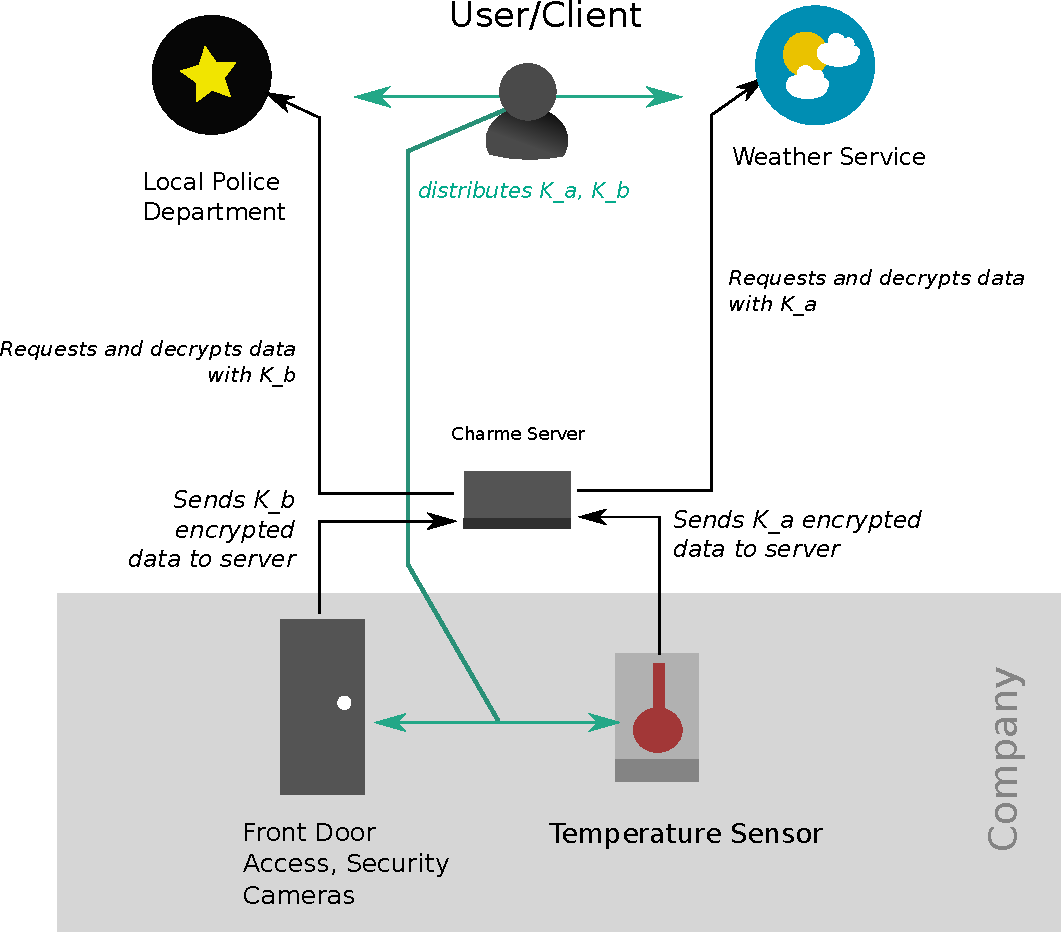
\includegraphics[width=120mm]{illustrations/iot.pdf}
%	\caption{K\_a, K\_b are keys shared between some service and the device. The data is encrypted so that only the user, the service and the device can see the data, but not the Charme server. Please note that for K\_b there must be some security mechanism  like timestamps to avoid replay attacks when the door is opened for example. \label{iot} }
%	\label{figContext}
%\end{figure}


\clearpage
\section{Terminology}

\begin{tabular}{p{4cm} p{10cm} }
          &  \\
\textbf{||} &  Concatenation Operator. For example $"a" || "b" \Leftrightarrow "ab" $ \\\\
\textbf{Conversation} & A sequence of messages belonging to two or more users  \\\\

\textbf{Encrypted Data Storage} & A JSON object in the cloud encrypted with an AES key that is only known by the user. Very vulnerable to replay attacks. \\\\

\textbf{Fastkey} & A symmetric key dependent on the passphrase. It is only known by the user itself, no other persons or servers. \\\\

\textbf{Key Update} &
A key update can happen after a new keyring is generated or someone has been removed of a conversation for example. In both cases we generate an updated key, but with a different protocol. \\\\


\textbf{Recrypt} &
Kind of neologism. Means to decrypt with an old key and encrypt with a new key. Maybe there is already another word for that...\\\\

\textbf{Revision} &
The version of the public key or edgekey. If a new key is established, it increases by 1.\\\\

\textbf{userId} &  An unique identifier for each person in the Charme network, similar to email. Example: ms@myserver.com
\end{tabular}


\clearpage
\section{Sources}
\printbibliography




  
\end{document}
